\section{Desenvolvimento}

% Slide 2: Estrutura de Pacotes
\begin{frame}{Desenvolvimento: Pacotes}
    \begin{itemize}
        \item Organização modular para encapsulamento de responsabilidades:
        \begin{itemize}
            \item \texttt{lexer}: Análise léxica e tokenização (feito com máquina de estados) .
            \item \texttt{parser}: Construção da AST com \textit{Pratt Parsing}.
            \item \texttt{walker}: Navegação e análise da AST.
            \item \texttt{checker}: Inferência de tipos e validações semânticas.
            \item \texttt{emitter}: Geração do código GLSL.
        \end{itemize}
    \end{itemize}
    \begin{figure}
        \centering
        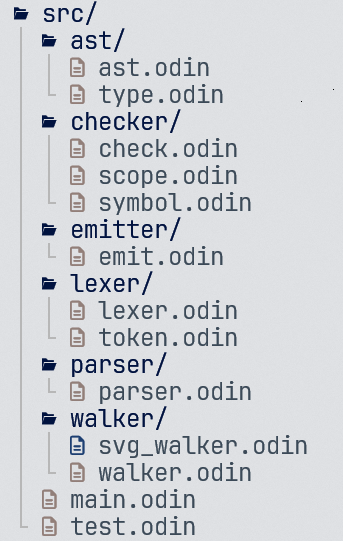
\includegraphics[scale=0.34]{./Imagens/package-structure.png}
        \caption{\small Estrutura de pacotes do compilador.}
    \end{figure}
\end{frame}


\begin{frame}{Desenvolvimento: Arquitetura do Compilador}
    \begin{figure}
        \centering
        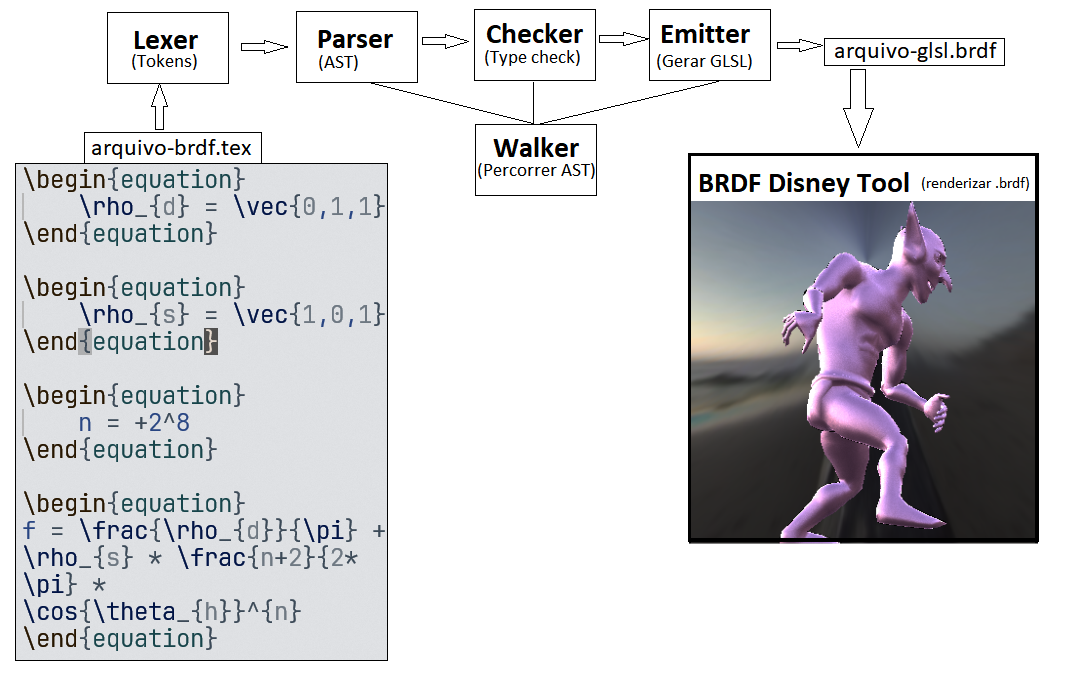
\includegraphics[scale=0.35]{./Imagens/new-arch-compiler.png}
        \caption{\small Estrutura geral da arquitetura do compilador.}
    \end{figure}
\end{frame}

% \begin{frame}{Desenvolvimento: Destaques}
%     \begin{itemize}
%         \item Análise sintática baseada em \textit{Pratt Parsing}, garantindo precisão e hierarquia nas expressões.
%         \item Funcionalidades do \texttt{walker}:
%         \begin{itemize}
%             \item Navegação genérica e preparação para verificações.
%             \item Suporte uniforme à travessia de nós.
%         \end{itemize}
%         \item Integração do \texttt{checker} com a tabela de símbolos para validações semânticas e consistência.
%         \item Geração de \textit{shaders} GLSL compatíveis com Disney BRDF Explorer.
%     \end{itemize}
% \end{frame}

\begin{frame}{Desenvolvimento: Erros de Compilação (1/3)}
    Exemplificando as verificações realizadas pelo compilador por meio dos possíveis erros que podem ser gerados. \\
    % \vspace{0.3cm}

       \textbf{Erro Léxico:}
       \begin{center}
           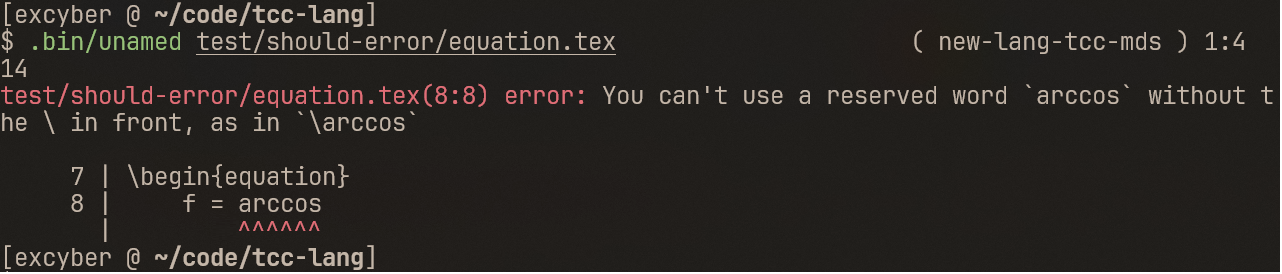
\includegraphics[width=\textwidth]{./Imagens/error-reserved-word.png}
           \small{Uso inválido de palavra reservada}
       \end{center}
       
       \textbf{Erro Sintático:}
       \begin{center}
           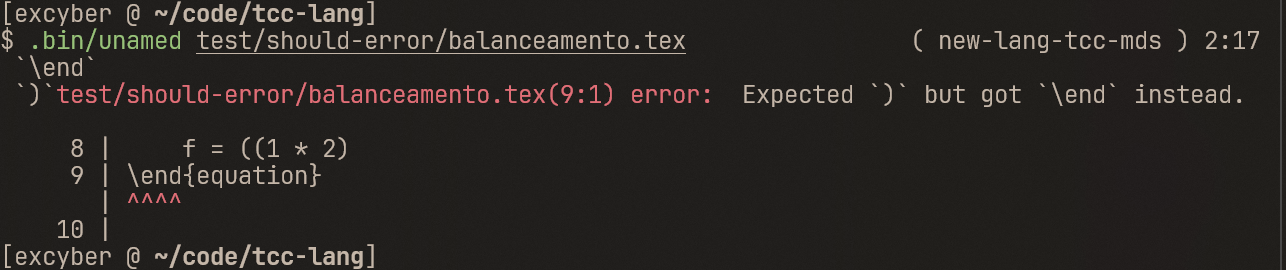
\includegraphics[width=\textwidth]{./Imagens/error-balanceamento.png}
           \small{Parênteses desbalanceados}
       \end{center}
\end{frame}

\begin{frame}{Erros de Compilação (2/3)}
       \textbf{Erro Sintático:}
       \begin{center}
           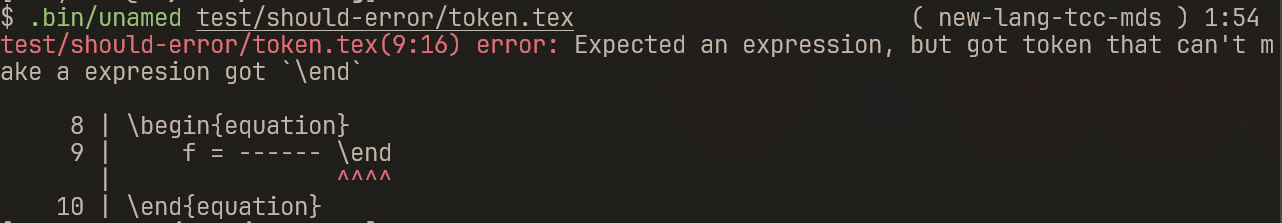
\includegraphics[width=\textwidth]{./Imagens/error-cant-make-expression.png}
           \small{Expressão matemática inválida}
       \end{center}
       
       \textbf{Erro Semântico:}
       \begin{center}
           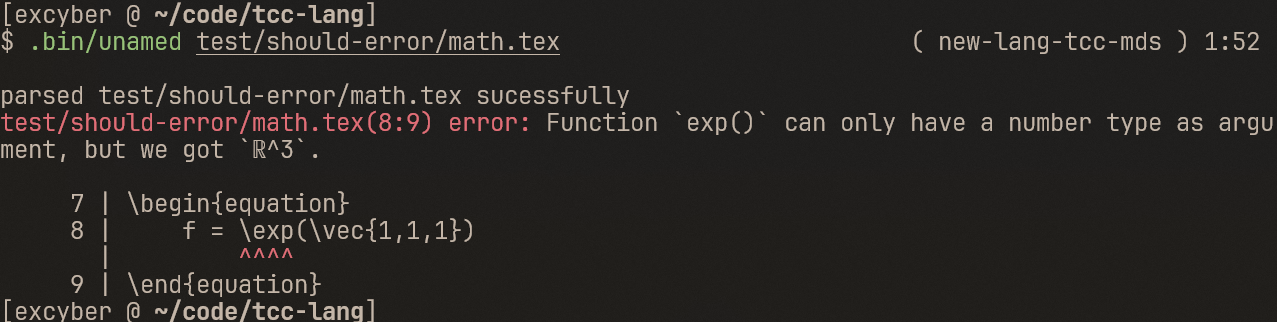
\includegraphics[width=\textwidth]{./Imagens/error-incompatible-types.png}
           \small{Tipos incompatíveis}
       \end{center}
\end{frame}

\begin{frame}{Erros de Compilação (3/3)}
       \textbf{Erro Semântico:}
       \begin{center}
           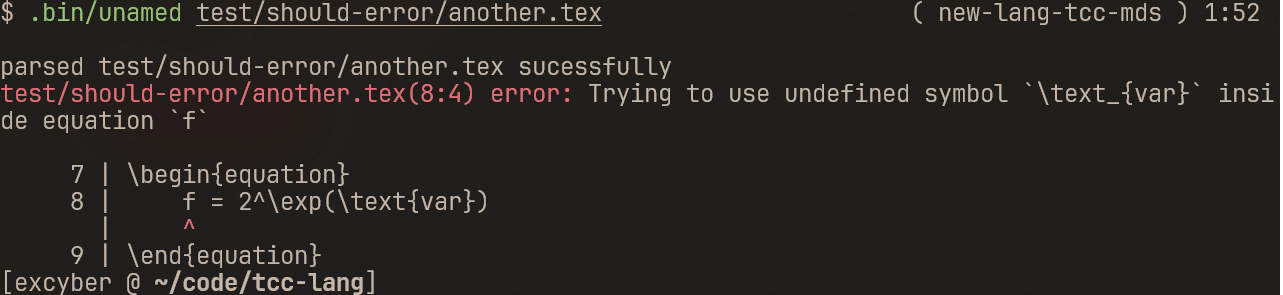
\includegraphics[width=\textwidth]{./Imagens/error-undefined-symbol.png}
           \small{Símbolo não definido}
       \end{center}
       
       \textbf{Erro Semântico:}
       \begin{center}
           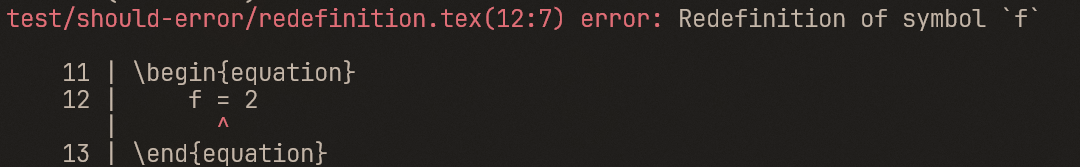
\includegraphics[width=\textwidth]{./Imagens/error-redefinition.png}
           \small{Redefinição de símbolo}
       \end{center}
\end{frame}
